\chapter{Introducción}
\label{cap:capitulo1}
\setcounter{page}{1}

\begin{flushright}
\begin{minipage}[]{10cm}
\emph{La meta de la humanidad es alcanzar la perfección, y la meta de los robots es ayudarnos a lograrla.}\\
\end{minipage}\\

Isaac Asimov, \textit{El hombre bicentenario}\\
\end{flushright}

\vspace{1cm}

Vivimos en una era donde la tecnología avanza a pasos agigantados, y la robótica está en el centro de esta revolución. Desde robots que construyen automóviles con una precisión milimétrica hasta aquellos que exploran planetas lejanos, la robótica ha dejado de ser ciencia ficción para convertirse en una herramienta fundamental en nuestra vida cotidiana. Estos sistemas inteligentes no solo automatizan tareas, sino que amplían las capacidades humanas, abriendo nuevas fronteras en la industria, la medicina, la exploración y más allá. En este contexto, la robótica móvil ha cobrado especial relevancia, ya que los robots autónomos se utilizan cada vez más en entornos que requieren desplazamientos controlados, como fábricas, almacenes, hospitales y hogares..\\

\section{Robótica}
\label{sec:miseccion} % etiqueta para luego referenciar esta sección

La robótica es la rama de la ingeniería y la ciencia que se dedica al diseño, construcción, operación y uso de robots, abarcando múltiples disciplinas. Un robot es una máquina programable diseñada para llevar a cabo tareas de forma autónoma o semiautónoma, siguiendo una serie de instrucciones preestablecidas o adaptándose a su entorno mediante el uso de sensores, controladores y actuadores. \\

La robótica comenzó como una idea visionaria en la antigüedad, con relatos y mitos de máquinas capaces de realizar tareas humanas. Sin embargo, los primeros desarrollos concretos no llegaron hasta el Renacimiento, cuando inventores como Leonardo da Vinci diseñaron autómatas mecánicos. \\

En el siglo XX, los primeros robots industriales, como el Unimate (Figura \ref{fig:unimate}), fueron diseñados para realizar tareas repetitivas en fábricas, lo que revolucionó la producción en masa. Estos robots no eran inteligentes, pero su capacidad para realizar trabajos peligrosos y repetitivos impulsó el desarrollo de la automatización en la industria. En paralelo, la ciencia ficción comenzó a popularizar la idea de robots humanoides con conciencia y emociones, aunque la tecnología no estaba ni cerca de eso.\\

\begin{figure} [h!]
  \begin{center}
    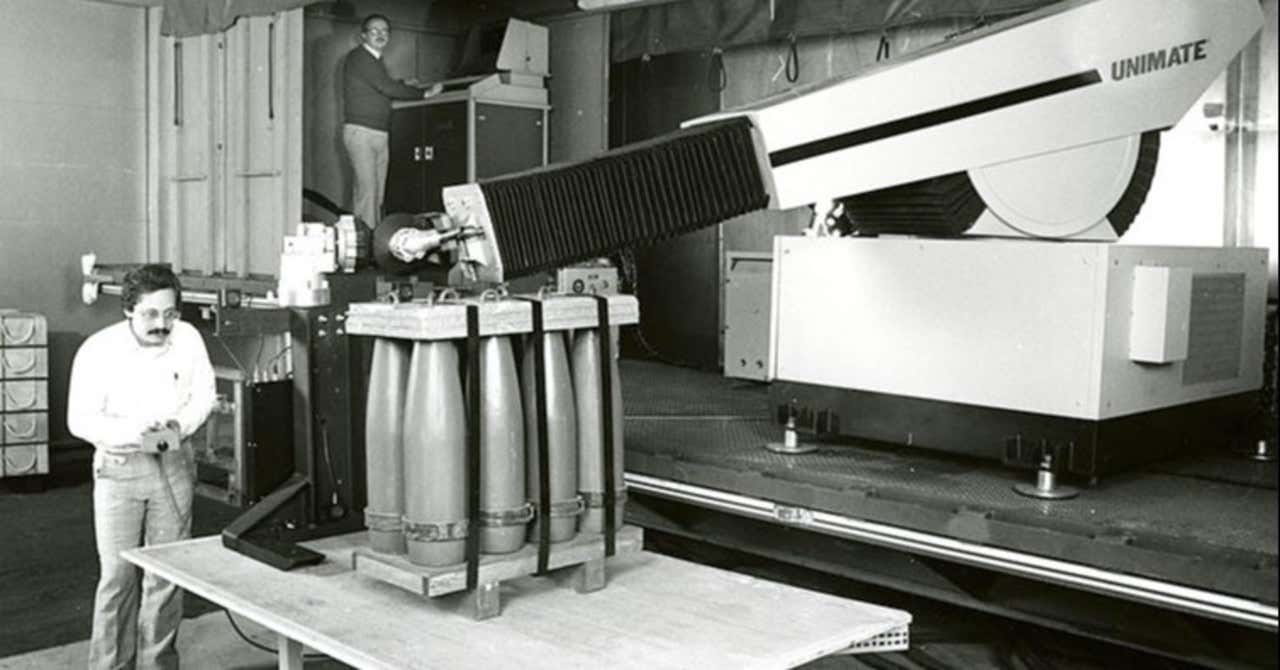
\includegraphics[width=8cm]{figs/unimate}
  \end{center}
  \caption{Robot Unimate.}
  \label{fig:unimate}
\end{figure}\




Con el avance de la informática en la segunda mitad del siglo XX, la robótica se integró cada vez más con la inteligencia artificial. Los robots dejaron de ser simples máquinas mecánicas para empezar a incorporar sensores y software que les permitían interactuar con su entorno de manera más flexible, como Shakey (Figura \ref{fig:shakey}), que podía tomar decisiones básicas sobre cómo moverse en su entorno.

\begin{figure} [H]
  \begin{center}
    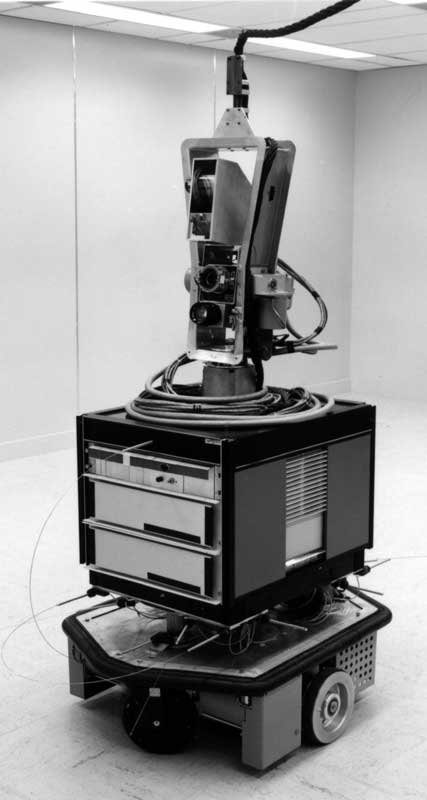
\includegraphics[scale=0.3]{figs/shakey}
  \end{center}
  \caption{Robot Shakey.}
  \label{fig:shakey}
\end{figure}\

En la actualidad se está aplicando en agricultura, logística, salud y exploración espacial, mostrando una evolución hacia máquinas más inteligentes, autónomas y adaptables. Hoy en día, los robots no solo ejecutan órdenes programadas, sino que también pueden aprender a partir de datos, tomar decisiones en tiempo real y adaptarse a entornos cambiantes. \\





\section{Robótica industrial}
\label{sec:segundaseccion}

La robótica industrial es el área de la robótica enfocada en el diseño, desarrollo y uso de robots en entornos industriales, cuyo objetivo es automatizar procesos productivos para mejorar la eficiencia, precisión, y seguridad en la fabricación de bienes. Los robots industriales son programables y están diseñados para realizar tareas repetitivas y a veces peligrosas para los humanos. Estos tipos de robots tienen alta precisión, velocidad y eficiencia y son versátiles. \\ \\ \\

\noindent\textbf{Manipuladores} 

Son un tipo de robot que se asemeja a un brazo humano y está diseñado para interactuar con su entorno a través de una serie de movimientos controlados. Estos robots están equipados con una serie de articulaciones que les permiten realizar tareas precisas y repetitivas, como agarrar, mover, ensamblar o manipular objetos. Suelen tener entre 3 y 7 grados de libertad que son las diferentes formas en las que el brazo puede moverse como rotaciones, desplazamientos lineales, etc. Un ejemplo de estos tipos son los robots Kuka\footnote{\url{https://www.kuka.com/es-es/productos-servicios/sistemas-de-robot/robot-industrial/kr-470-pa}} (Figura \ref{fig:kuka}) y los Yamaha\footnote{\url{https://global.yamaha-motor.com/business/robot/lineup/ykxg/large/}} (Figura \ref{fig:yamaha}).


\begin{figure}[h!]
  \begin{minipage}{0.48\textwidth}
    \centering
    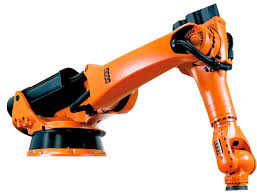
\includegraphics[width=6.5cm]{figs/kuka}
    \caption{Robot KUKA.}
    \label{fig:kuka}
  \end{minipage}
  \hfill
  \begin{minipage}{0.48\textwidth}
    \centering
    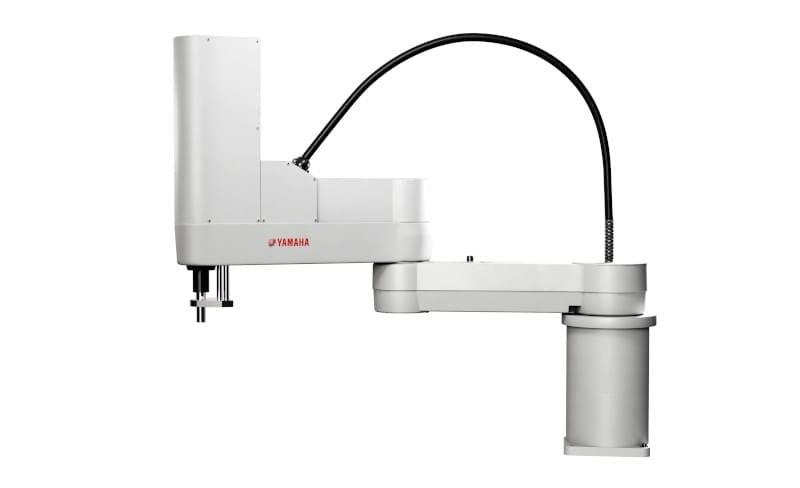
\includegraphics[width=8cm]{figs/yamaha}
    \caption{Robot Yamaha.} 
    \label{fig:yamaha}
  \end{minipage}
\end{figure}

\noindent\textbf{Cartesianos} 

Estos robots se mueven a lo largo de tres ejes lineales ortogonales (X, Y, Z), como el DL ROB2X-1200(Figura \ref{fig:cartesiano}), siguiendo el sistema de coordenadas cartesianas. Tiene una estructura sencilla y es adecuado para realizar movimientos precisos y repetitivos en trayectorias rectas. Se usan normalmente en tareas de pick and place o impresión 3D, entre otras.
 


\begin{figure} [h!]
  \begin{center}
    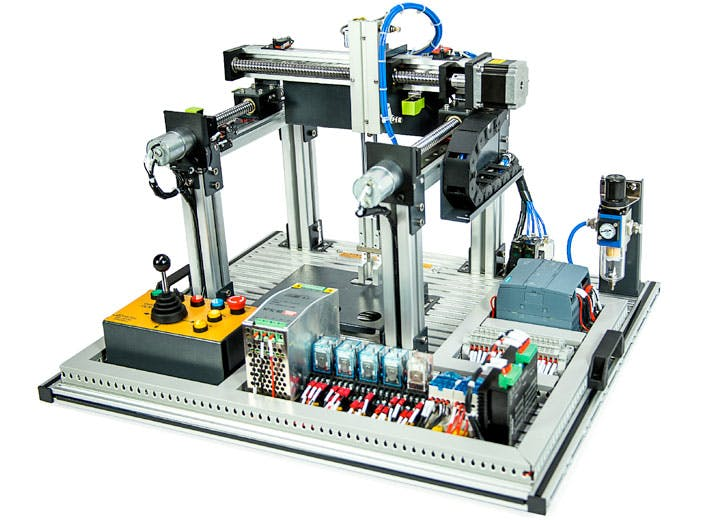
\includegraphics[width=6.5cm]{figs/cartesiano}
  \end{center}
  \caption{DL ROB2X-1200.}
  \label{fig:cartesiano}
\end{figure}\

\noindent\textbf{Delta} 




Se caracterizan por su diseño de brazos paralelos a la base y su capacidad para realizar movimientos rápidos y precisos en un espacio tridimensional, como por ejemplo el ABB IRB 360\footnote{\url{https://new.abb.com/products/robotics/robots/delta-robots/irb-360}} (Figura \ref{fig:delta}). Este tipo de robot se utiliza principalmente en aplicaciones de manipulación y ensamblaje debido a su alta velocidad y su capacidad para manejar objetos livianos con gran precisión. 

\begin{figure} [h!]
  \begin{center}
    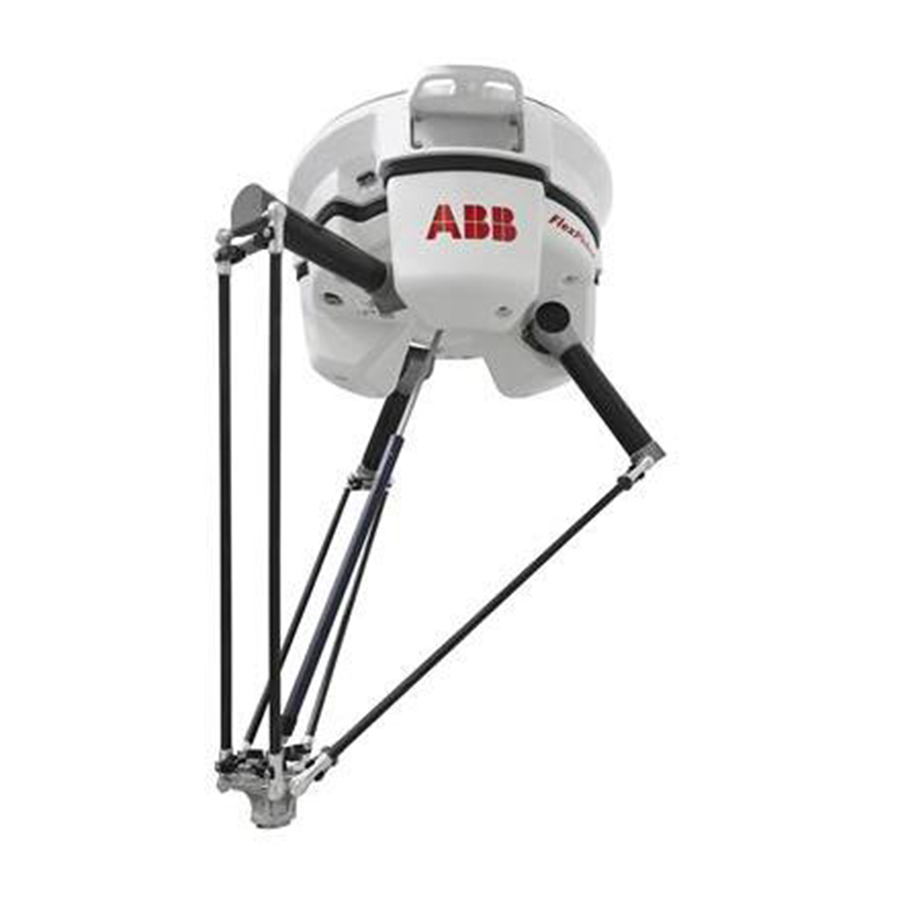
\includegraphics[width=8cm]{figs/delta}
  \end{center}
  \caption{ABB IRB 360.}
  \label{fig:delta}
\end{figure}\


La robótica es un campo que avanza rápidamente, con el objetivo de desarrollar máquinas inteligentes y autónomas capaces de llevar a cabo tareas cada vez más sofisticadas. Este progreso, liderado en gran medida por la robótica industrial, no solo impacta en los procesos productivos, sino que también aumenta la demanda de profesionales capacitados en este ámbito. Para satisfacer esta necesidad, la robótica educativa juega un papel crucial, permitiendo que las personas adquieran habilidades prácticas y conocimientos tecnológicos desde una etapa temprana. De esta forma, ambos enfoques se complementan para preparar a las nuevas generaciones para un entorno cada vez más automatizado. En la siguiente sección veremos en profundidad el alcance de la robótica educativa.


\section{Robótica educativa}
\label{sec:terceraseccion}


La robótica educativa se ha vuelto crucial en los últimos tiempos ya que prepara a las nuevas generaciones para un futuro tecnológico, fomentando habilidades clave en los institutos; como las matemáticas, la programación, la resolución de problemas y la electrónica, que es lo que se conoce como \hyperlink{STEM}{STEM} (Science, Technology, Engineering and Mathematics). También reduce brechas educativas y capacita a los estudiantes para enfrentar los retos de un mundo cada vez más automatizado.\\

La participación creciente de los robots móviles en nuestra vida cotidiana ha impulsado la creación de programas educativos que incorporan actividades prácticas de robótica en escuelas primarias y secundarias, promoviendo habilidades como la creatividad fomentando además el trabajo en equipo.\\


A principios de los 2000 algunas universidades y centros de formación empezaron a ofrecer cursos y talleres enfocados en la robótica educativa y se comenzaron a crear los primeros programas de robótica dirigidos a estudiantes, utilizando kits como LEGO Mindstorms (Figura \ref{fig:lego}), que facilitaban el aprendizaje de la programación y la construcción de robots.

\begin{figure} [h!]
  \begin{center}
    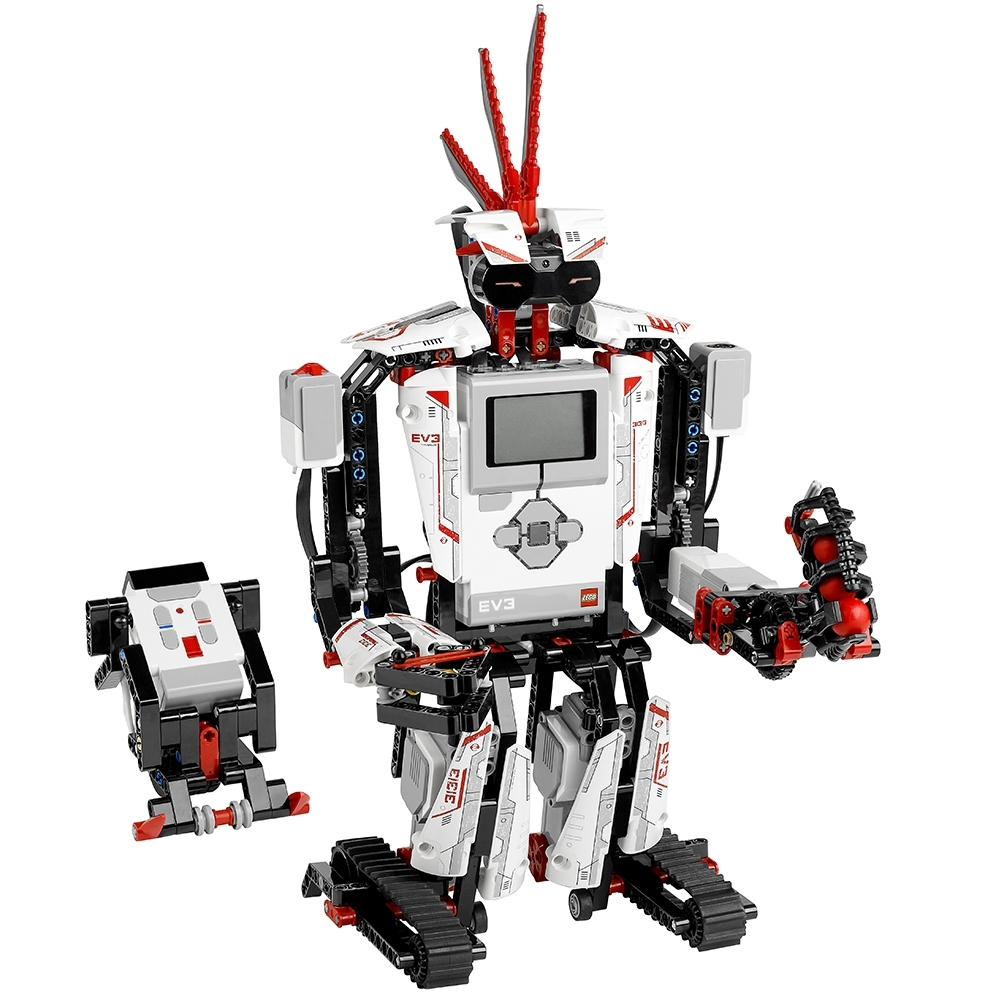
\includegraphics[width=8cm]{figs/lego}
  \end{center}
  \caption{LEGO MINDSTORMS EV3.}
  \label{fig:lego}
\end{figure}\



La creación de competiciones como la First Lego League \footnote{\url{https://firstlegoleague.soy/}} (Figura \ref{fig:First Lego League}) y la RoboCup Junior \footnote{\url{https://junior.robocup.org/}} (Figura \ref{fig:RoboCup Junior}), que llegaron a España a mediados de la década de 2010, dio un gran impulso a la robótica en las aulas y los estudiantes tuvieron la oportunidad de programar, diseñar y construir robots de distintos tipos para poder competir.



\begin{figure}[h!]
  \begin{minipage}{0.48\textwidth}
    \centering
    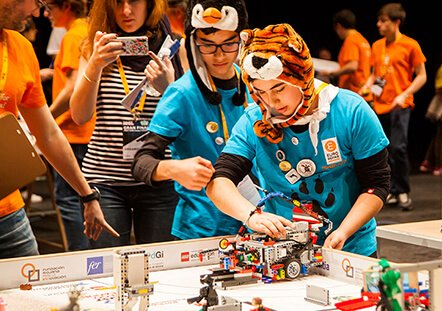
\includegraphics[width=6.5cm]{figs/first-lego-league.jpg}
    \caption{First Lego League.}
    \label{fig:First Lego League}
  \end{minipage}
  \hfill
  \begin{minipage}{0.48\textwidth}
    \centering
    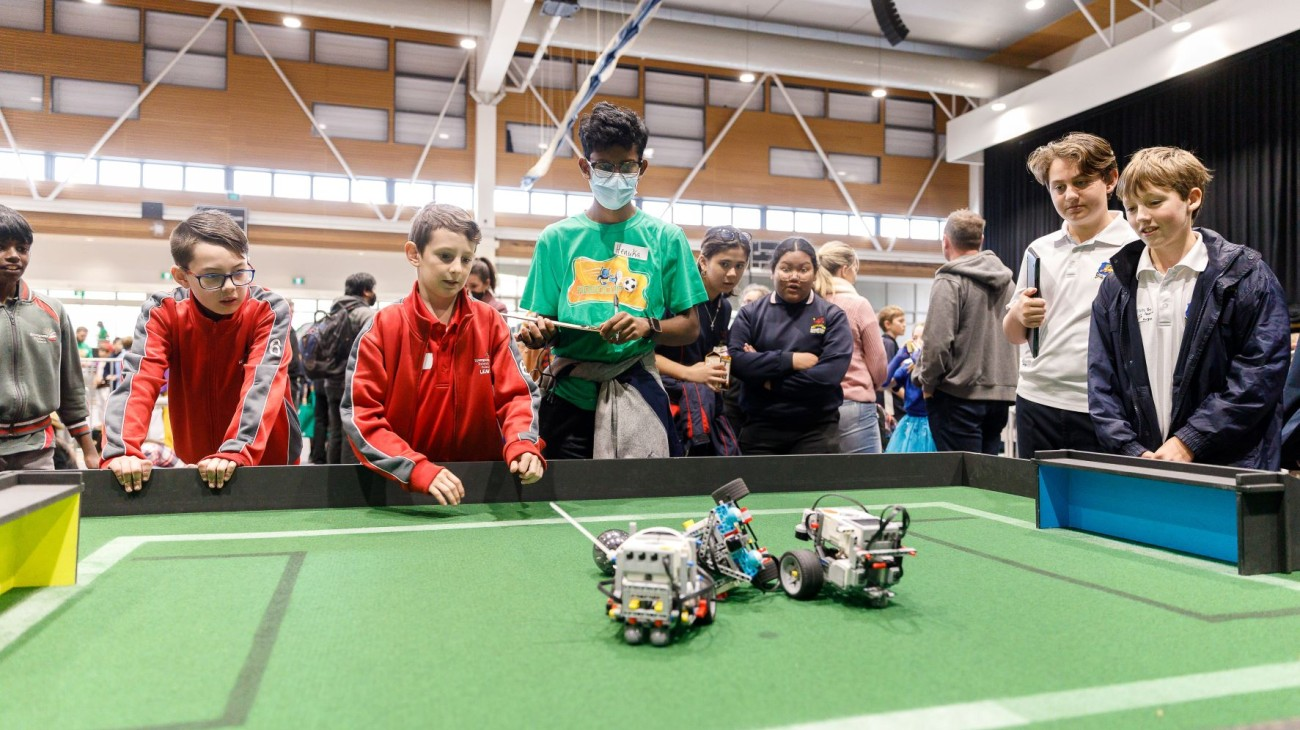
\includegraphics[width=8cm]{figs/RoboCup_junior.jpg}
    \caption{RoboCup Junior.} 
    \label{fig:RoboCup Junior}
  \end{minipage}
\end{figure}


Según el decreto \cite{Madrid}, se añadió la asignatura Tecnología, Programación y Robótica, en la cual los alumnos podrían estudiar los contenidos acerca de Scratch\footnote{\url{https://scratch.mit.edu/}} (Figura \ref{fig:scratch}) que utiliza bloques gráficos que los usuarios pueden arrastrar y soltar para crear programas, eliminando la necesidad de escribir código de texto y Arduino. 

\begin{figure} [h!]
  \begin{center}
    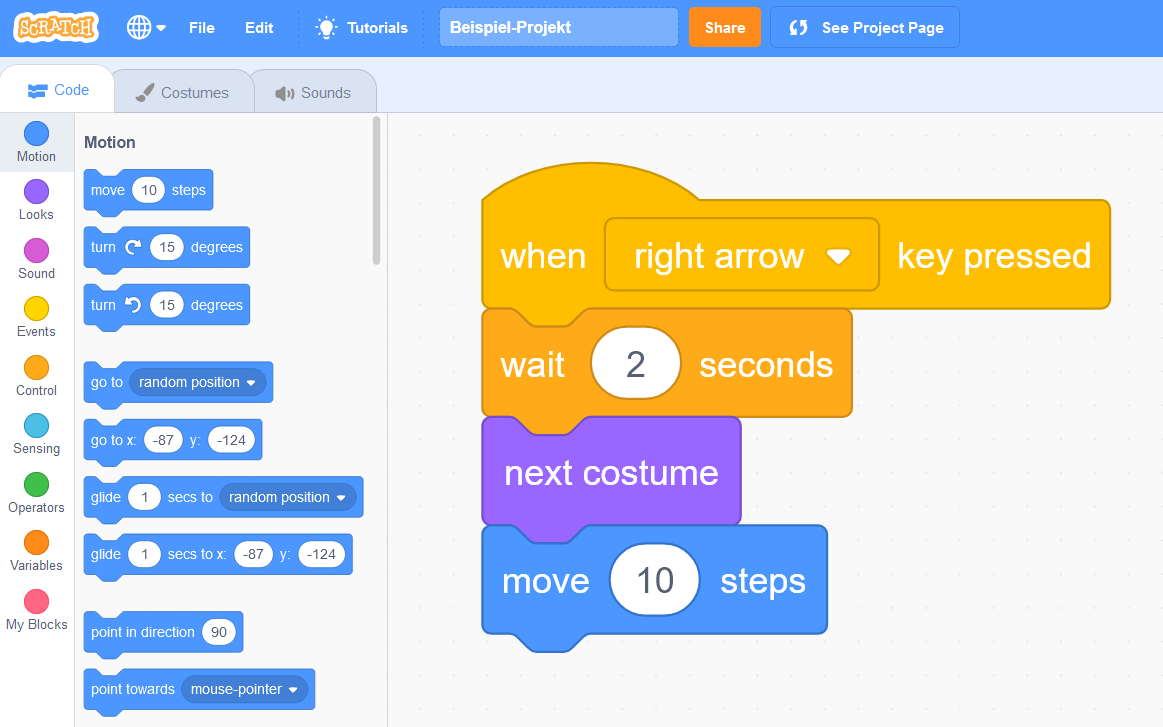
\includegraphics[width=8cm]{figs/scratch.png}
  \end{center}
  \caption{Programación con Scratch.}
  \label{fig:scratch}
\end{figure}\

Esta última tecnología debía de ser de bajo coste debido a la alta demanda y se usaron placas Arduino\footnote{\url{https://www.arduino.cc/}} (Figura \ref{fig:arduino}) y Raspberry Pi\footnote{\url{https://www.raspberrypi.com/}}(Figura \ref{fig:raspberry}), con las cuales se podían controlar sensores y actuadores de un robot de una manera más sencilla e interactiva para el usuario, aunque también tienen ciertas limitaciones a la hora de poder añadir algún hardware más complejo como un LIDAR para Arduino por ejemplo o algún actuador como motores con más potencia que requiera algún robot ya que en Raspberry, como mucho, se podrían controlar motores como las de las impresoras 3D, lo cual nos limita bastante a la hora de trabajar con robots de mayores dimensiones.


\begin{figure}[H]
  \begin{minipage}{0.48\textwidth}
    \centering
    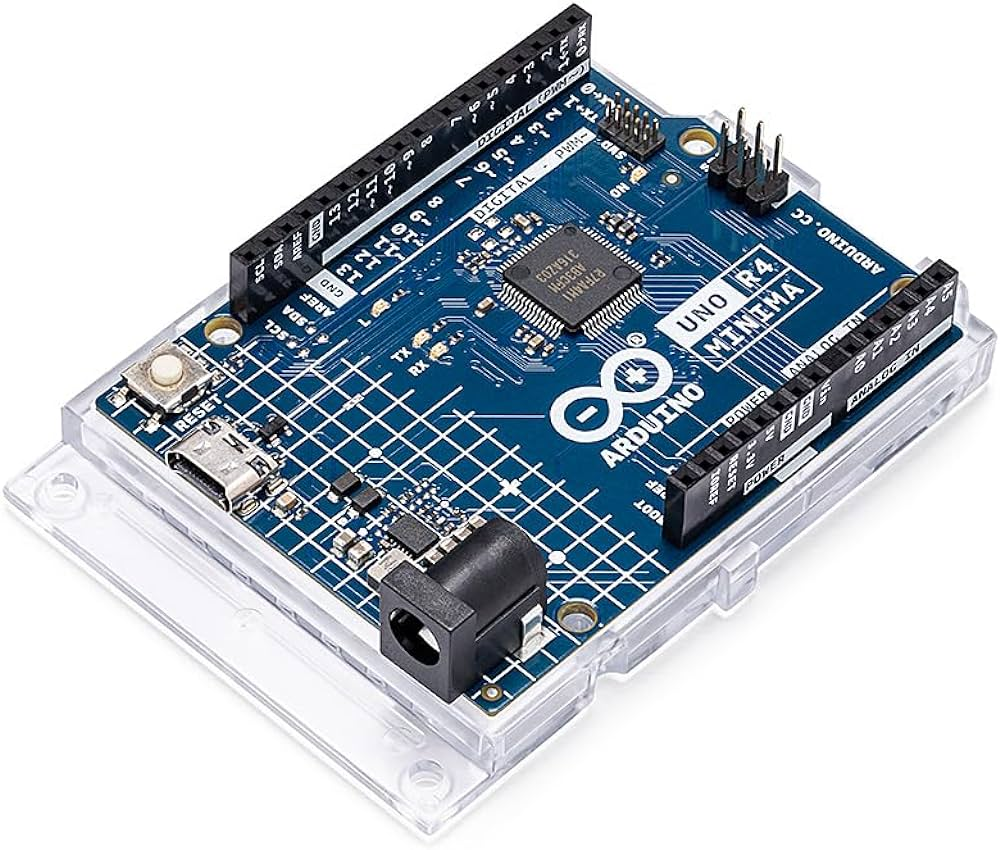
\includegraphics[width=6.5cm]{figs/arduino_uno.jpg}
    \caption{Arduino UNO.}
    \label{fig:arduino}
  \end{minipage}
  \hfill
  \begin{minipage}{0.48\textwidth}
    \centering
    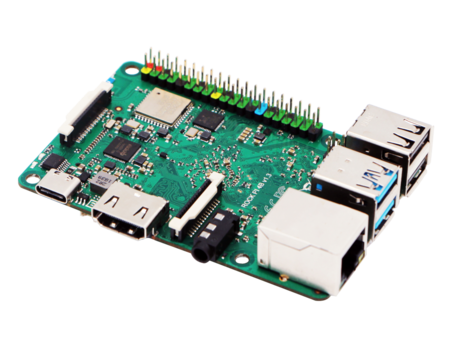
\includegraphics[width=7.2cm]{figs/raspberry4.png}
    \caption{Raspberry 4, Modelo B.} 
    \label{fig:raspberry}
  \end{minipage}
\end{figure}

Por eso se creó \hyperlink{ROS}{ROS} (Robot Operating System): un middleware estándar robótico que está estructurado como se indica en la Figura \ref{fig:ros}, para abordar varios desafíos y necesidades en la robótica moderna, especialmente en entornos de investigación y desarrollo de robots complejos cuyo propósito principal era proporcionar una infraestructura flexible y modular que permita a los desarrolladores e investigadores crear, integrar y controlar sistemas robóticos avanzados de manera más eficiente. El paso de \hyperlink{ROS}{ROS} a ROS2 fue un cambio necesario para abordar una serie de limitaciones y mejorar varios aspectos el soporte para sistemas en tiempo real, la seguridad y fiabilidad, soporte multiplataforma, etc.


\begin{figure} [h!]
  \begin{center}
    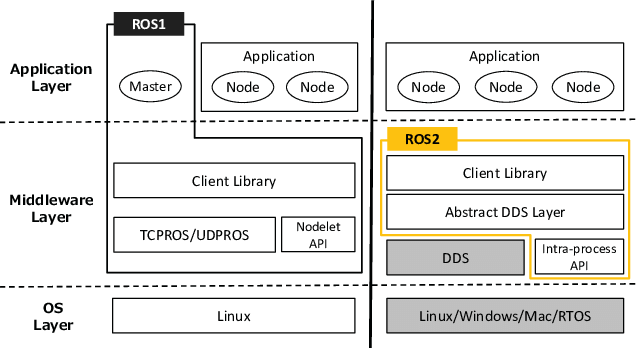
\includegraphics[width=10cm]{figs/ros.png}
  \end{center}
  \caption{Arquitectura de ROS y ROS2.}
  \label{fig:ros}
\end{figure}\

Con este middleware hay un salto muy grande en términos de aprendizaje ya que no es suficiente con conocer el lenguaje de programación sino que hay que entender todo el entorno de esta plataforma(estructuras de datos, programación modular, comunicaciones...), por lo que sería necesaria una conexión entre estos niveles de aprendizaje como por ejemplo alguna asignatura más o algún programa en la etapa de Bachillerato o Secundaria enfocada en este aspecto.\\

A medida que la robótica educativa ha evolucionado, los progresos en inteligencia artificial han abierto nuevas oportunidades para mejorar las capacidades y la autonomía de los robots. En este sentido, el aprendizaje automático ha comenzado a desempeñar un papel fundamental, permitiendo así que los robots no sigan solo instrucciones preprogramadas, sino que también aprendan de su entorno, optimicen su comportamiento y tomen decisiones basadas en datos. Esta combinación de robótica y aprendizaje automático no solo amplía el alcance de la educación \hyperlink{STEM}{STEM}, sino que también introduce a los estudiantes en conceptos clave de la inteligencia artificial, allanando el camino para sistemas más autónomos y sofisticados.


\section{Machine learning}


Dentro de la inteligencia artificial, se encuentra el ámbito del aprendizaje automático o Machine Learning. Un modelo de aprendizaje automático consiste en un archivo inteligente que se ha condicionado con un algoritmo para poder aprender patrones específicos en diferentes conjuntos de datos y así proporcionar información y predicciones a partir de ellos.\\

Al crear un modelo de aprendizaje automático, se define la respuesta que se desea capturar y se establecen los parámetros con los que debe funcionar y de los que debe aprender el modelo. Cuando se habilita un modelo de aprendizaje automático a través de un algoritmo, este puede empezar aprendiendo el conjunto de datos y descubriendo la información. Cuanta más información obtiene el modelo, más puede utilizar el conocimiento para acelerar y mejorar el descubrimiento.\\ 

Aunque los ordenadores no cuentan con la capacidad de razonar y aprender con la experiencia, los algoritmos que alimentan estos modelos funcionan para simular esa experiencia en la medida de lo posible. Con los parámetros y ajustes de los algoritmos, los modelos pueden replicar el aprendizaje de la experiencia y eso facilita un profundo nivel de análisis y predicciones que resultarían imposibles de otro modo. \\

El algoritmo que emplean para aprender se ha creado utilizando datos de entrenamiento y de prueba, y genera una estimación en los datos partiendo de un patrón. Estos datos pueden estar etiquetados o no; y, si lo están, quiere decir que el modelo lo debe identificar en su justa medida. Después, la función de error evaluará la precisión del modelo sobre la decisión que ha tomado y se observará cuánto de preciso es el modelo sobre esos datos. Por último, se optimizarán los modelos en la medida de lo posible ajustando los diferentes parámetros para que se pueda adaptar mejor al conjunto de datos de entrenamiento hasta poder cumplir un umbral de precisión.\\ 



Existen diferentes tipos de aprendizaje en Machine Learning: 

\begin{itemize}
 \item \textit{Aprendizaje supervisado.} En este método, los conjuntos de datos están etiquetados y se conoce la salida y el modelo se entrena con los datos de la salida conocida; es decir, para entrenar el al algoritmo para que reconozca fotos de manzanas, hay que transmitirle fotos etiquetadas como manzanas (regresión lineal, árboles de decisión, etc.).
 \item \textit{Aprendizaje no supervisado.} Es un modelo que usa datos sin etiquetar con el objetivo de aprender patrones y no cuenta con un conjunto entrenado previamente. El algoritmo en este caso aprende de los datos sin intervención humana y los categoriza en grupos según los atributos, por lo que es bueno para la coincidencia de patrones (mínimos cuadrados, K-means, etc.).
 \item \textit{Aprendizaje semisupervisado.} En este modelo, solo se etiquetan algunos datos y el algoritmo debe determinar cómo organizar y estructurar los datos para lograr un resultado conocido. Por ejemplo, al modelo de aprendizaje automático se le dice que el resultado es una pera, pero solo algunos datos de entrenamiento están etiquetados como una pera.
\end{itemize}\

El aprendizaje automático ha impulsado avances importantes en la autonomía y la capacidad de decisión de los robots, lo cual ha facilitado la creación de sistemas más inteligentes y adaptativos. Sin embargo, la implementación de estas tecnologías a menudo se ve limitada por los altos costos del hardware y la infraestructura computacional necesarios para entrenar y ejecutar modelos complejos. En este contexto, la robótica de bajo costo se presenta como una alternativa para tener acceso a estas innovaciones, permitiendo así que investigadores, educadores y entusiastas experimenten con inteligencia artificial sin requerir grandes inversiones. Gracias al uso de componentes asequibles y plataformas de código abierto, es posible integrar algoritmos de aprendizaje automático en sistemas robóticos económicos, ampliando su uso en educación, investigación y desarrollo.

 
\label{sec:cuartaseccion}


\section{Robótica de bajo coste}
\label{sec:quintaseccion}

La robótica de bajo coste está enfocada en el diseño, desarrollo y uso de sistemas robóticos que son accesibles económicamente, usando componentes de bajo coste pero sin eliminar la funcionalidad básica con el objetivo de reducir la complejidad de los sistemas ya existentes. Esto ha tenido un gran impacto en áreas como la educación y la investigación académica.\\

El uso de la impresión 3D y el software libre, junto con el uso de componentes económicos, ha dado paso a la creatividad de los usuarios para crear piezas con un propósito específico personalizadas a un precio más asequible que si las hubieran tenido que comprar ya hechas.\\


Todo esto ha fomentado la filosofía \hyperlink{DIY}{DIY}, que promueve la personalización y creación propia de objetos y proyectos de forma autónoma. Todo esto sin tener que depender de productos comerciales ya construidos previamente.\\

Un ejemplo de esta área es el robot Makeblock mBot\footnote{\url{https://www.makeblock.com/pages/mbot-robot-kit}} (Figura \ref{fig:mbot-2}) desarrollado por la empresa china Makeblock, que se usaba en las escuelas para enseñar programación y electrónica y era compatible con muchos sensores y accesorios, además de poder usar microcontroladores como el de Arduino, por lo que era ideal para aportar soluciones creativas en este ámbito.

\begin{figure} [H]
  \begin{center}
    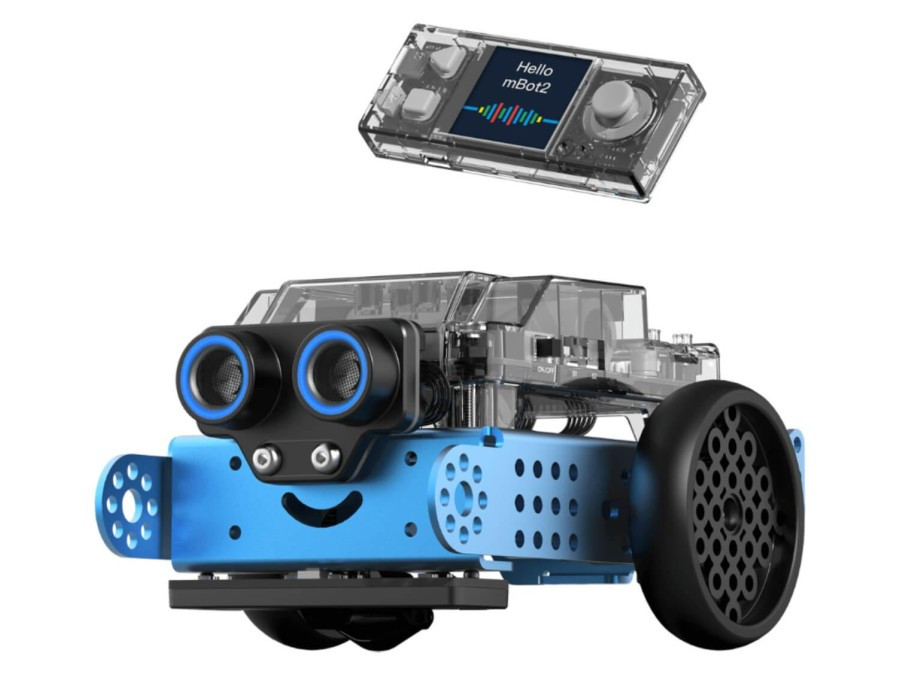
\includegraphics[width=6cm]{figs/mbot-2.jpg}
  \end{center}
  \caption{Makeblock mBot.}
  \label{fig:mbot-2}
\end{figure}\


Otro ejemplo de robot de bajo coste ampliamente usado en educación es el TurtleBot\footnote{\url{https://www.turtlebot.com/turtlebot3/}} (Figura \ref{fig:turtlebot}). Este fue desarrollado por la empresa Willow Garage, los creadores de \hyperlink{ROS}{ROS}, y el objetivo era ofrecer una plataforma robótica económica y accesible. Por ello, las universidades empezaron a usarlo, ya que las instituciones educativas enfrentaban problemas en cuanto al presupuesto, por lo que este robot era el ideal para poder experimentar con \hyperlink{ROS}{ROS} de una manera más asequible para los estudiantes, ya que el presupuesto era relativamente barato en comparación con otras plataformas robóticas que había en el momento.

\begin{figure} [H]
  \begin{center}
    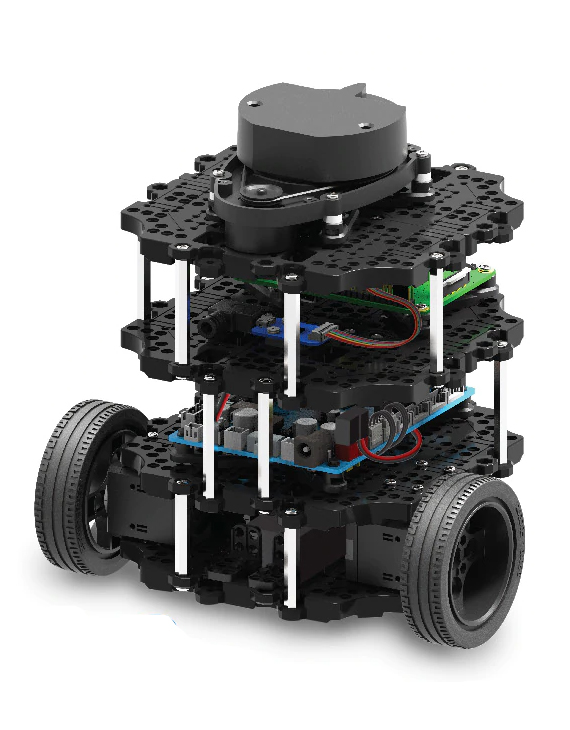
\includegraphics[scale=0.25]{figs/turtlebot3burguer.jpg}
  \end{center}
  \caption{TurtleBot 3 Burger.}
  \label{fig:turtlebot}
\end{figure}\


El presente trabajo está enfocado en la fabricación y programación de un robot móvil de bajo coste diseñado para que sea fácil de usar a partir de diferentes componentes hardware y piezas diseñadas en 3D, siguiendo así la filosofía \hyperlink{DIY}{DIY}. Mediante diferentes técnicas y procedimientos, como los modelos de aprendizaje automáticos, se podrá obtener una estimación precisa de cuántos dispositivos de red son necesarios para que el robot pueda localizarse en interiores de la mejor manera posible y a partir de una interfaz \hyperlink{HRI}{HRI} amena, se podrá controlar al robot por comandos de voz mediante técnicas avanzadas. Finalmente, se presentarán diferentes métodos para que el robot pueda navegar por diferentes trayectorias siguiendo un camino hacia un objetivo claro a partir de los comandos de voz y para que sea portable a diferentes entornos de la manera más asequible posible. Uno de los objetivos es lograr que funcionen todos estos métodos y procedimientos en una CPU de baja capacidad de cómputo, como la Raspberry, y que sea portable a diferentes entornos en interiores de la manera más asequible posible. En el siguiente capítulo se presentarán diferentes investigaciones y estudios previos que tienen una cierta similitud con el diseño y la programación interna del robot que se ha fabricado.

\vspace{15cm} % Espacio vertical de 1 cm







